%!TEX root = ../main.tex
\chapter{Extraction of noise hits for simulation.}
\label{appendix:noise}

The AHCAL operates in auto-trigger during data taking. Due to this feature, noise hits can't be extracted like the previous CALICE physics prototypes which were extracted by sending external triggers to the detector between beam spills. Moreover, if no validation signal is provided by the trigger scintillators to the chip, hits that are stored in the chip are removed.

One solution to this problem is to use real data events to extract noise hits. It is can be efficiently done using muon runs because a track is present in the calorimeter due to the muon. By removing the identified muon track and keeping remaining hits, noise hits can be extracted. Muon runs from 24647 to 24656 are used for the extraction of noise hits. The table \ref{table:noise_sel} shows the cuts applied for event selection.

The track found in the selected event is removed and the remaining hits are considered as noise hits. Initially, the time of the noise hits is in TDC unit. To get an approximation time distribution of noise hits, the time of a noise hit is randomly shifted by a flat distribution between 500 and 3500 ns. This acts as a time reference for these hits to give a good description of the noise time distribution. The figures \ref{fig:noise_energy} and \ref{fig:noise_time} show the energy and time distribution of noise hits.

\begin{figure}[htbp!]
	\centering
	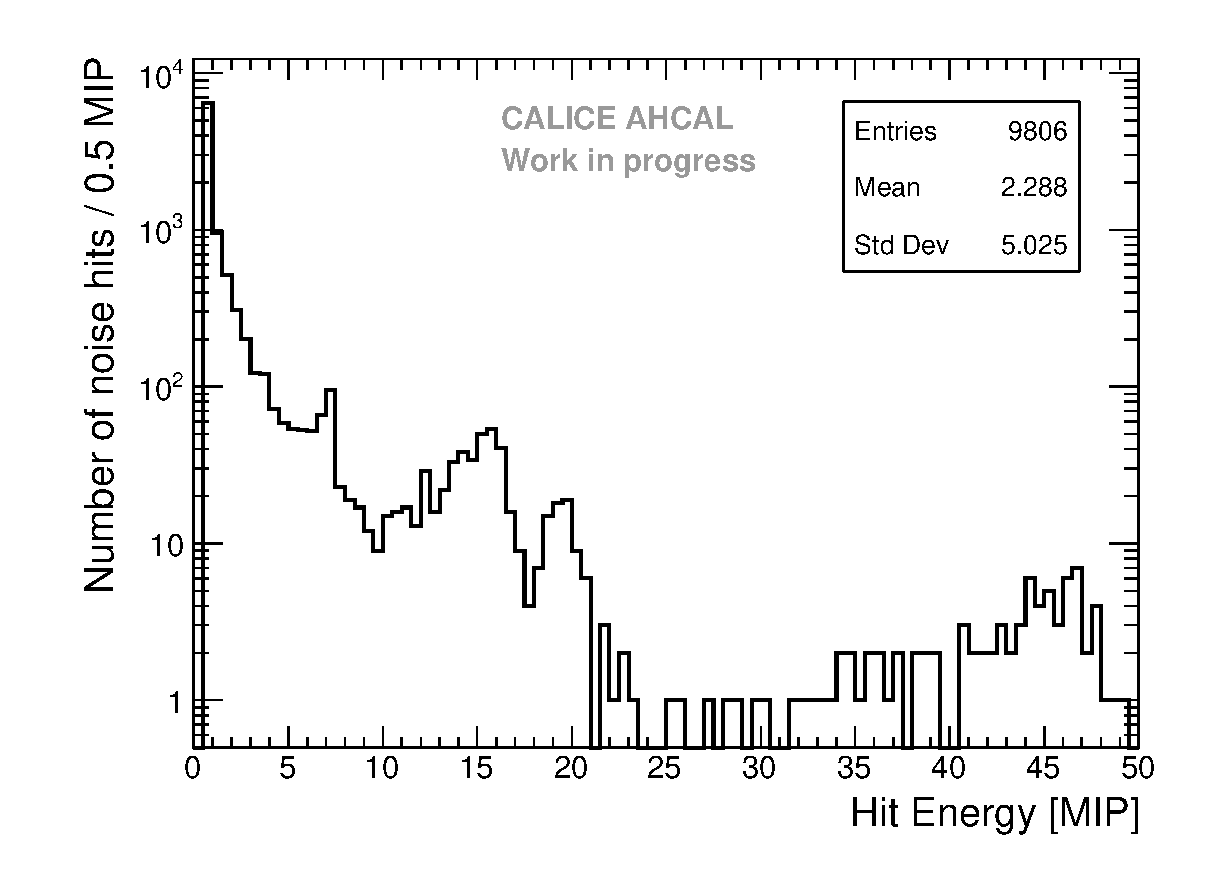
\includegraphics[width=0.7\linewidth]{../Thesis_Plots/Timing/Muons/Plots/Noise_Energy_Flat.eps}
	\caption{Hit energy distribution of the extracted noise hits. Most of the hits have an energy below 2 MIPs although a tail is visible to high energies.} \label{fig:noise_energy}
\end{figure}

\begin{figure}[htbp!]
	\centering
	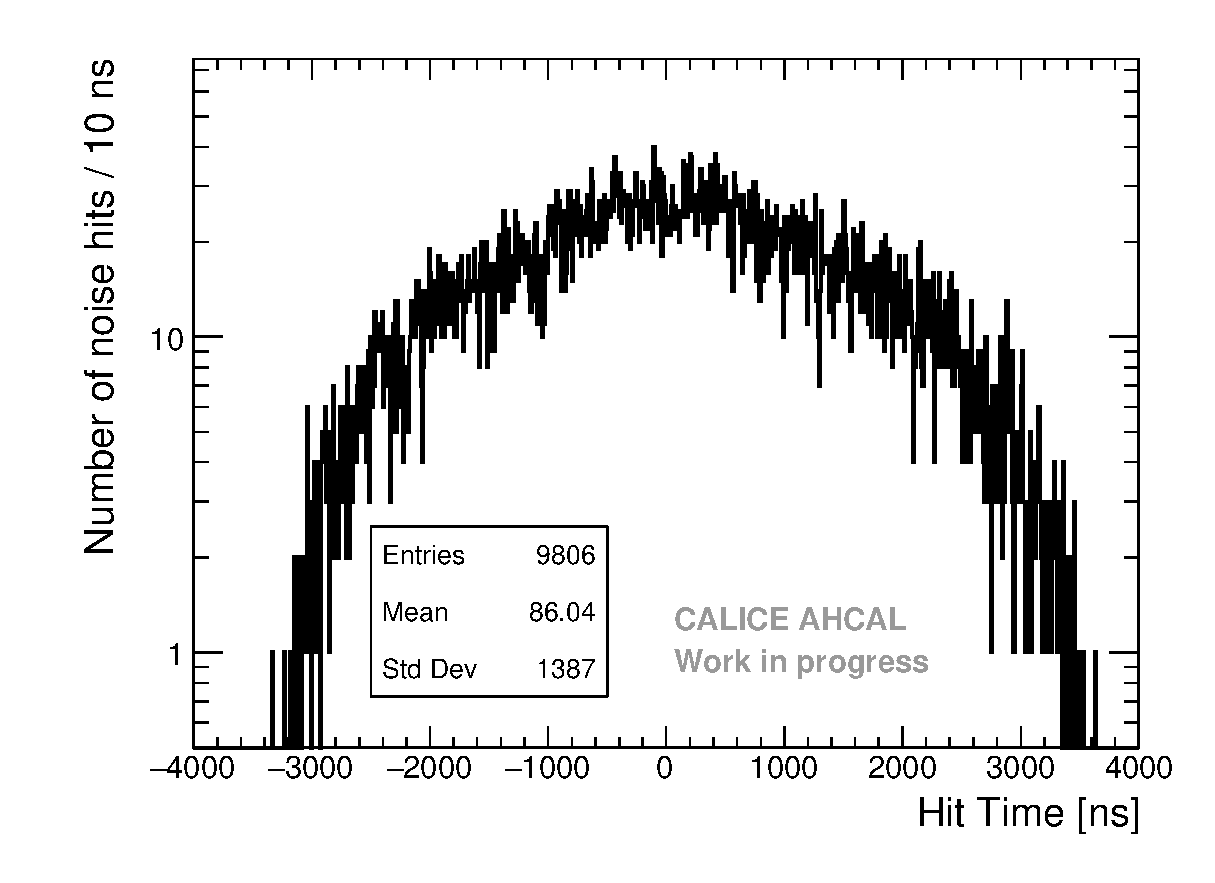
\includegraphics[width=0.7\linewidth]{../Thesis_Plots/Timing/Muons/Plots/Noise_Time_Flat.eps}
	\caption{Time distribution of the extracted noise hits. The description of the shape of the time distribution is important for the simulation.} \label{fig:noise_time}
\end{figure}

Most of the fraction of noise hits have an energy under 2 MIPs. Higher hit energies can be seen and they may be due to delta electrons from muon tracks. However, it is not expected to have a great impact on timing. The introduction of noise for timing is very important to compare data and simulation especially for pions where a late tail is present.
